%2_limits.tex
%notes for the course Algorithms COMS10007 taught at the University of Bristol
%2017_18 Conor Houghton conor.houghton@bristol.ac.uk

%To the extent possible under law, the author has dedicated all copyright 
%and related and neighboring rights to these notes to the public domain 
%worldwide. These notes are distributed without any warranty. 

\documentclass[11pt,a4paper]{scrartcl}
\typearea{12}
\usepackage{graphicx}
%\usepackage{pstricks}
\usepackage{listings}
\usepackage{color}
\lstset{language=C}
\pagestyle{headings}
\markright{COMS10007 1\_limits (d) - Conor}
\definecolor{dark-gray}{gray}{0.25}
\begin{document}

\section*{2: Limits}

Limits are the mathematical framework for deciding where a function is
going as its argument approaches some value. In the case of algorithmic
complexity, we are interested in where $T(n)$, the run time, is going,
as $n$ gets large so here we will look at limits at infinity. The
limit is a part of mathematics where the intuition is probably more
straight forward than the definition, nonetheless here we will look at
the formal definition. This is useful not so much for this course,
largely we will be able to calculate the limits we need using simple
methods, but because it is something that is useful to know in the
future and it is interesting because it demonstrates a powerful way of
proving things that is common in some types of mathematics.

\subsection*{Informal idea}

If we write
\begin{equation}
\lim_{x\rightarrow \infty}f(x)=c
\end{equation}
where $f(x)$ is some function and $c$ a constant, we mean that $f(x)$
heads towards infinity it gets close to $c$. Take, for example
\begin{equation}
f(x) = \frac{1}{x}
\end{equation}
it is easy to see that 
\begin{equation}
\lim_{x\rightarrow \infty}\frac{1}{x}=0
\end{equation}
because the bigger $x$ is, the smaller $1/x$ is, so $1/x$ is heading for zero. Now, lets consider 
\begin{equation}
f(x)=\frac{4x^2+2x+1}{2x^2+3}
\end{equation}
Well by dividing above and below by $x^2$ we have
\begin{equation}
\lim_{x\rightarrow \infty}\frac{4x^2+2x+1}{2x^2+3}=
\lim_{x\rightarrow \infty}\frac{4+2/x+1/x^2}{2+3/x^2}=
\lim_{x\rightarrow \infty}\frac{4}{2}=2
\end{equation}
because the $2/x$, $3/x^2$ and so on are getting smaller and smaller
as $x$ gets larger so we can replace them by zeros inside the limit.

Of course, many functions just get bigger and bigger, or more and more
negative, as $x$ goes to infinity, for these we say the limit is plus
or minus infinity, so, for example
\begin{equation}
\lim_{x\rightarrow \infty} x=\infty
\end{equation}
and
\begin{equation}
\lim_{x\rightarrow \infty} (-x)=-\infty
\end{equation}

\subsection*{Formal definition}

The informal approach to limits makes sense until you think about it,
then it starts to get confusing: what do we mean by \lq{}$x$
approaches infinity\rq{}, what do we mean by \lq{}gets close
to\rq{}. The formal definition of the limit explains all of this. 

We say
\begin{equation}
\lim_{x\rightarrow \infty}f(x)=c
\end{equation}
if for all $\delta>0$ there exists an $x_0$ such that for all $x>x_0$
we have $|f(x)-c|<\delta$.

What this definition is doing is this: no matter what standard of
\lq{}close to\rq{} you set, that is, if you regard \lq{}close to
$c$\rq{} as meaning within $\delta$ of $c$ then no matter how small a
value of $\delta$ you choose, then $f(x)$ will eventually end up that
close; the $x_0$ is the eventually, you can make $f(x)$ lie within
$\delta$ of $c$ by choosing a high enough $x_0$.

This style of definition is refered to as an epsilon-delta-box. You
might ask where the epsilon is, the delta, of course, is the $\delta$:
$\epsilon$ is used for limits that aren't at infinity, 
\begin{equation}
\lim_{x\rightarrow a}f(x)=c
\end{equation}
which we aren't looking at here. The epsilon plays a similar role to
the $x_0$ here.

There is also a definition of an infinite limit:
We say
\begin{equation}
\lim_{x\rightarrow \infty}f(x)=\infty
\end{equation}
if for all $y>0$ there exists an $x_0$ such that for all $x>x_0$
we have $f(x)>y$. Thus, no matter what you consider big, that is, no matter how large a $y$ you choose, $f(x)$ will eventually be bigger than it. Finally
\begin{equation}
\lim_{x\rightarrow \infty}f(x)=-\infty
\end{equation}
if for all $y<0$ there exists an $x_0$ such that for all $x>x_0$
we have $f(x)<y$.

\subsection*{How to work out limits}

Limits actually have nice properties:
\begin{equation}
\lim_{x\rightarrow \infty}[f(x)\pm g(x)]=\lim_{x\rightarrow \infty}f(x)\pm \lim_{x\rightarrow \infty}g(x)
\end{equation}
where, following the usual convention, you take the $+$ in both
$\pm$s, or the minus in both. If everything is finite:
\begin{equation}
\lim_{x\rightarrow \infty}[f(x)g(x)]=\left[\lim_{x\rightarrow \infty}f(x)\right]\left[\lim_{x\rightarrow \infty}g(x)\right]
\end{equation}
and
\begin{equation}
\lim_{x\rightarrow \infty}\frac{f(x)}{g(x)}=\frac{\lim_{x\rightarrow \infty}f(x)}{\lim_{x\rightarrow \infty}g(x)}
\end{equation}
Although we didn't mention it, we used these rules earlier when doing
\begin{equation}
\lim_{x\rightarrow \infty}\frac{4x^2+2x+1}{2x^2+3}=
\lim_{x\rightarrow \infty}\frac{4+2/x+1/x^2}{2+3/x^2}=
\lim_{x\rightarrow \infty}\frac{4}{2}=2
\end{equation}
What we actually did was 
\begin{equation}
\lim_{x\rightarrow \infty}\frac{4+2/x+1/x^2}{2+3/x^2}=
\frac{\lim_{x\rightarrow \infty}(4+2/x+1/x^2)}{\lim_{x\rightarrow \infty}(2+3/x^2)}=
\lim_{x\rightarrow \infty}\frac{4}{2}
\end{equation}
and, for example
\begin{equation}
\lim_{x\rightarrow \infty} (4+2/x+1/x^2)=\lim_{x\rightarrow \infty} 4+\lim_{x\rightarrow \infty}2/x+\lim_{x\rightarrow \infty}1/x^2
\end{equation}

The other method for calculating limits is l'H\^{o}pital's rule. If 
\begin{equation}
\lim_{x\rightarrow \infty}f(x)=\lim_{x\rightarrow \infty}g(x)=\infty
\end{equation}
then
\begin{equation}
\lim_{x\rightarrow \infty}\frac{f(x)}{g(x)}=\frac{\lim_{x\rightarrow \infty} f(x)}{\lim_{x\rightarrow \infty} g(x)}
\end{equation}
doesn't tell us anything since the right hand side is just infinity
over infinity and we did say above the business with products and
fractions only applies if everything is finite. However in this case a
rule called l'H\^{o}pital's rule.\footnote{Which was discovered by
  Johann Bernoulli; he gave l'H\^{o}pital permission to include it in
  a book and was then \textsl{very} annoyed when he found that people
  thought it was l'H\^{o}pital's idea.} L'H\^{o}pital's rule says that
\begin{equation}
\lim_{x\rightarrow \infty}\frac{f(x)}{g(x)}=\lim_{x\rightarrow \infty}\frac{f'(x)}{g'(x)}
\end{equation}
where 
\begin{equation}
f'(x)=\frac{df}{dx}(x)
\end{equation}
and similar for $g'(x)$. In other words, if the top and the bottom
both have infinity limits then differentiating the top and the bottom
doesn't change the limit. 

You might wonder why you'd want to differenciate the top and the
bottom, in fact that can sometimes simplify the limit; this is
important for an example we need for algorithmic complexity, calculating
\begin{equation}
\lim_{x\rightarrow \infty}\frac{\log_2{x}}{x}
\end{equation}
Now, $\lim_{x\rightarrow\infty}\log{x}=\infty$ and $\lim_{x\rightarrow \infty}x=\infty$ so we can apply l'H\^{o}pital's rule:
\begin{equation}
\lim_{x\rightarrow \infty}\frac{\log_2{x}}{x}=\lim_{x\rightarrow \infty}\frac{1/x}{1}=\lim_{x\rightarrow \infty}\frac{1}{x}=0
\end{equation}
This tells us that although $\log_2{x}$ goes to infinity it goes to
infinity slower than $x$.  This is illustrated in a plot,
Fig.~\ref{fig_log}. Here, by the way, in line with standard
practice in computer science, we are using the log to the base two, in
fact changing bases only causes a change of an overall constant, see
Table~\ref{math_logs} for a reminder of the properties of the log.

\begin{table}
\color{dark-gray}
The logarithm is the opposite of the exponent: if
\begin{equation}
a^b=c
\end{equation}
then 
\begin{equation}
\log_a{c}=b
\end{equation}
or, written in one line
\begin{equation}
a^{\log_a{c}}=c
\end{equation}
All the laws of logs can be worked out from the laws of
exponents. Hence, since $a^0=1$ we have $\log_a{1}=0$. In a similar
way, other rules of logs can be deduced like
\begin{eqnarray}
\log_a{c_1c_2}&=&\log_a{c_1}+\log_a{c_2}\cr
\log_a{\frac{c_1}{c_2}}&=&\log_a{c_1}-\log_a{c_2}\cr
\log_a c^d&=&d\log_a c
\end{eqnarray}
and so on.

As for the change of base, let $b=\log_{a_1}{c}$ so $a_1^{b}=c$. Now take the log to the base $a_2$ of both sides
\begin{equation}
b\log_{a_2}a_1=\log_{a_2}{c}
\end{equation}
and then solve for $b$
\begin{equation}
b=\frac{\log_{a_2}c}{\log_{a_2}a_1}
\end{equation}
and, substituting back the formula for $b$
\begin{equation}
\log_{a_1}{c}=\frac{\log_{a_2}c}{\log_{a_2}a_1}
\end{equation}
Thus we see, that changing bases is just a matter of a
multiplicative factor. For example, to change from base $e$ to base two
\begin{equation}
\log_{2}{x}=\frac{\log_e{x}}{\log_e{2}}\approx\frac{\log_e{x}}{0.6931}
\end{equation}
Common bases are $\log_2{x}$ used in computer science, $\log_e{x}$
sometimes written $\ln{x}$ used in mathematics and $\log_{10}{x}$ used
in chemistry. The base two is used because of its link to bits and
also, as we will see, because of its relationship with algorithms that
divide data into two piles. The natural log $\ln{x}$ is used where
differential equations are common since
\begin{equation}
\frac{d}{dx}\ln{x}=\frac{1}{x}
\end{equation}
\caption{A reminder about logarithms. This is a quick summary of some of the laws of logs.\label{math_logs}}
\color{black}
\end{table}

\begin{figure}
% GNUPLOT: LaTeX picture with Postscript
\begingroup
  \makeatletter
  \providecommand\color[2][]{%
    \GenericError{(gnuplot) \space\space\space\@spaces}{%
      Package color not loaded in conjunction with
      terminal option `colourtext'%
    }{See the gnuplot documentation for explanation.%
    }{Either use 'blacktext' in gnuplot or load the package
      color.sty in LaTeX.}%
    \renewcommand\color[2][]{}%
  }%
  \providecommand\includegraphics[2][]{%
    \GenericError{(gnuplot) \space\space\space\@spaces}{%
      Package graphicx or graphics not loaded%
    }{See the gnuplot documentation for explanation.%
    }{The gnuplot epslatex terminal needs graphicx.sty or graphics.sty.}%
    \renewcommand\includegraphics[2][]{}%
  }%
  \providecommand\rotatebox[2]{#2}%
  \@ifundefined{ifGPcolor}{%
    \newif\ifGPcolor
    \GPcolorfalse
  }{}%
  \@ifundefined{ifGPblacktext}{%
    \newif\ifGPblacktext
    \GPblacktexttrue
  }{}%
  % define a \g@addto@macro without @ in the name:
  \let\gplgaddtomacro\g@addto@macro
  % define empty templates for all commands taking text:
  \gdef\gplbacktext{}%
  \gdef\gplfronttext{}%
  \makeatother
  \ifGPblacktext
    % no textcolor at all
    \def\colorrgb#1{}%
    \def\colorgray#1{}%
  \else
    % gray or color?
    \ifGPcolor
      \def\colorrgb#1{\color[rgb]{#1}}%
      \def\colorgray#1{\color[gray]{#1}}%
      \expandafter\def\csname LTw\endcsname{\color{white}}%
      \expandafter\def\csname LTb\endcsname{\color{black}}%
      \expandafter\def\csname LTa\endcsname{\color{black}}%
      \expandafter\def\csname LT0\endcsname{\color[rgb]{1,0,0}}%
      \expandafter\def\csname LT1\endcsname{\color[rgb]{0,1,0}}%
      \expandafter\def\csname LT2\endcsname{\color[rgb]{0,0,1}}%
      \expandafter\def\csname LT3\endcsname{\color[rgb]{1,0,1}}%
      \expandafter\def\csname LT4\endcsname{\color[rgb]{0,1,1}}%
      \expandafter\def\csname LT5\endcsname{\color[rgb]{1,1,0}}%
      \expandafter\def\csname LT6\endcsname{\color[rgb]{0,0,0}}%
      \expandafter\def\csname LT7\endcsname{\color[rgb]{1,0.3,0}}%
      \expandafter\def\csname LT8\endcsname{\color[rgb]{0.5,0.5,0.5}}%
    \else
      % gray
      \def\colorrgb#1{\color{black}}%
      \def\colorgray#1{\color[gray]{#1}}%
      \expandafter\def\csname LTw\endcsname{\color{white}}%
      \expandafter\def\csname LTb\endcsname{\color{black}}%
      \expandafter\def\csname LTa\endcsname{\color{black}}%
      \expandafter\def\csname LT0\endcsname{\color{black}}%
      \expandafter\def\csname LT1\endcsname{\color{black}}%
      \expandafter\def\csname LT2\endcsname{\color{black}}%
      \expandafter\def\csname LT3\endcsname{\color{black}}%
      \expandafter\def\csname LT4\endcsname{\color{black}}%
      \expandafter\def\csname LT5\endcsname{\color{black}}%
      \expandafter\def\csname LT6\endcsname{\color{black}}%
      \expandafter\def\csname LT7\endcsname{\color{black}}%
      \expandafter\def\csname LT8\endcsname{\color{black}}%
    \fi
  \fi
  \setlength{\unitlength}{0.0500bp}%
  \begin{picture}(7200.00,5040.00)%
    \gplgaddtomacro\gplbacktext{%
      \csname LTb\endcsname%
      \put(726,704){\makebox(0,0)[r]{\strut{} 0}}%
      \put(726,1383){\makebox(0,0)[r]{\strut{} 0.5}}%
      \put(726,2061){\makebox(0,0)[r]{\strut{} 1}}%
      \put(726,2740){\makebox(0,0)[r]{\strut{} 1.5}}%
      \put(726,3418){\makebox(0,0)[r]{\strut{} 2}}%
      \put(726,4097){\makebox(0,0)[r]{\strut{} 2.5}}%
      \put(726,4775){\makebox(0,0)[r]{\strut{} 3}}%
      \put(858,484){\makebox(0,0){\strut{} 1}}%
      \put(1849,484){\makebox(0,0){\strut{} 1.5}}%
      \put(2840,484){\makebox(0,0){\strut{} 2}}%
      \put(3831,484){\makebox(0,0){\strut{} 2.5}}%
      \put(4821,484){\makebox(0,0){\strut{} 3}}%
      \put(5812,484){\makebox(0,0){\strut{} 3.5}}%
      \put(6803,484){\makebox(0,0){\strut{} 4}}%
      \put(3830,154){\makebox(0,0){\strut{}$x$}}%
    }%
    \gplgaddtomacro\gplfronttext{%
      \csname LTb\endcsname%
      \put(1450,4602){\makebox(0,0)[r]{\strut{}$\log_2{x}$}}%
      \csname LTb\endcsname%
      \put(1450,4382){\makebox(0,0)[r]{\strut{}$x-1$}}%
    }%
    \gplbacktext
    \put(0,0){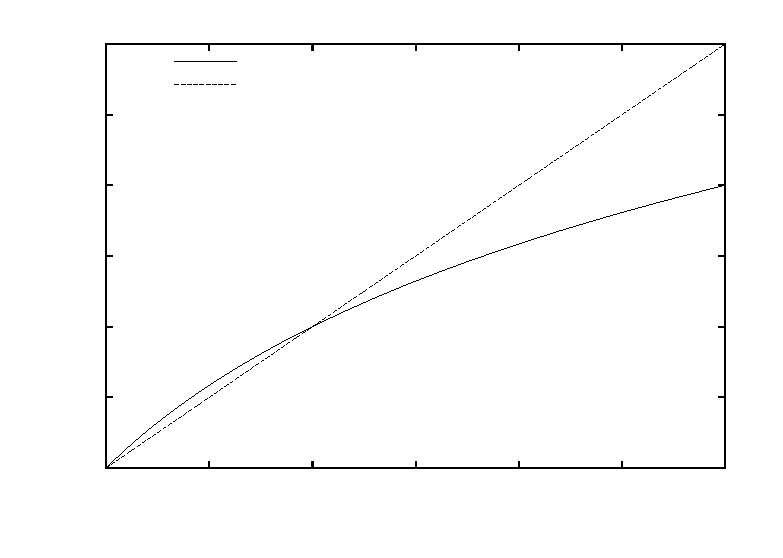
\includegraphics{log.eps}}%
    \gplfronttext
  \end{picture}%
\endgroup

\caption{This shows $\log_2{x}$ and $x-1$ plots for $x\in[1,4]$, the one has been taken from $x$ to make them easier to compare, the key point is that the $x$ grows faster.\label{fig_log}}
\end{figure}


\subsection*{Relationship to big-Oh}

Recall the definition of $O(g(n)$, called \lq{}big oh\rq{} of
$g(n)$, is
\begin{equation}
O(g(n))=\{f(n)| \exists n_0>0\in \mathbf{ N}\mbox{ and }c>0\in \mathbf{R}\mbox{ with }|f(n)|\le c|g(n)|\,\forall n\ge n_0\}
\end{equation}
You can see that the definition of $O(g(n))$ has this wrapped up in
it, if says
\begin{equation}
f(n)\in O(g(n))\iff \lim_{n\rightarrow \infty}\frac{f(n)}{g(n)}<\infty
\end{equation}
Or, put another way, either $f(n)$ goes to infinity slower than
$g(n)$, or at the same speed.

Lets look at the example we saw before:
\begin{equation}
T(n)=5n^2+n+6
\end{equation}
we can see
\begin{equation}
\lim_{n\rightarrow \infty}\frac{5n^2+n+6}{n^2}=5<\infty
\end{equation}
so $T(n)\in O(n^2)$.


\end{document}

